\subsection{Parametrization of the \texorpdfstring{$\pth$}{pTH} spectra as a function of Higgs boson couplings}


The gluon fusion cross section can be expressed as a second-degree polynomial in terms of the couplings to all the particles that are included in the loop~\cite{higgshunter} (see also Section~\ref{sec:production-decay}):
% 
\begin{linenomath*}
\begin{equation}
\label{eq:kappa-parametrization}
\Delta\sigma^{\ggh}_i = \sum_a \sum_b A_{ab,\,i} \kappa_a \kappa_b 
\,,
\end{equation}
\end{linenomath*}
% 
where the index $a$ ($b$) refers to particle $a$ ($b$), index $i$ refers to bin $i$ in the $\pth$ spectrum, and $A_{ab,\,i}$ is a coefficient of the parametrization.
% 
Typically the coefficients are only non-negligible for a limited number of particles.
% 
The variations of $\Delta\sigma^{\ggh}_i$ are precomputed by the theorists for given values of the couplings; what rests is to find the coefficients $A_{ab,\,i}$.
% 
Assuming there are no statistical fluctuations in the input spectra, finding the coefficients can be done by simple matrix inversion.
% 
Taking for example three simultaneous variations of $\kappat$ and $\cg$, $(\kappa_{\tquark,\,1}, c_{\gluon,\,1})$, $(\kappa_{\tquark,\,2}, c_{\gluon,\,2})$, and $(\kappa_{\tquark,\,3}, c_{\gluon,\,3})$, one can write for a single bin in the $\pth$ spectrum:
% 
\begin{linenomath*}
\begin{equation}
\left[\begin{array}{c}
\Delta\sigma_1 \\
\Delta\sigma_2 \\
\Delta\sigma_3
\end{array}\right]
    =
    \left[\begin{array}{ccc}
        \kappa_{\tquark,\,1}^2  &  c_{\gluon,\,1}^2   &  \kappa_{\tquark,\,1} c_{\gluon,\,1} \\
        \kappa_{\tquark,\,2}^2  &  c_{\gluon,\,2}^2   &  \kappa_{\tquark,\,2} c_{\gluon,\,2} \\
        \kappa_{\tquark,\,3}^2  &  c_{\gluon,\,3}^2   &  \kappa_{\tquark,\,3} c_{\gluon,\,3}
        \end{array}\right]
    %
    \left[\begin{array}{c}
        A \\
        B \\
        C
        \end{array}\right]
    \,,
\end{equation}
\end{linenomath*}
% 
where $A$, $B$, and $C$ are the coefficients of the parametrization.
% 
The coefficients can then conveniently be retrieved:
% 
\begin{linenomath*}
\begin{equation}
\left[\begin{array}{c}
A \\
B \\
C
\end{array}\right]
=
    \left[\begin{array}{ccc}
        \kappa_{\tquark,\,1}^2  &  c_{\gluon,\,1}^2   &  \kappa_{\tquark,\,1} c_{\gluon,\,1} \\
        \kappa_{\tquark,\,2}^2  &  c_{\gluon,\,2}^2   &  \kappa_{\tquark,\,2} c_{\gluon,\,2} \\
        \kappa_{\tquark,\,3}^2  &  c_{\gluon,\,3}^2   &  \kappa_{\tquark,\,3} c_{\gluon,\,3}
        \end{array}\right]^{-1}
    %
    \left[\begin{array}{c}
        \Delta\sigma_1 \\
        \Delta\sigma_2 \\
        \Delta\sigma_3
        \end{array}\right]
    \,.
\end{equation}
\end{linenomath*}
% 
As the statistical fluctuations are negligible for the precomputed spectra from Refs.~\cite{Grazzini:2017szg,Grazzini:2016paz}, this methods works well; the precomputed spectra and the parametrization at the same values of the couplings are plotted in Fig.~\ref{fig:theories_ktcgkb}, for simultaneous variations of $\kappat$ and $\cg$ (left) and for $\kappat$ and $\kappab$ (right).


\begin{figure}[hbtp]
  \begin{center}
    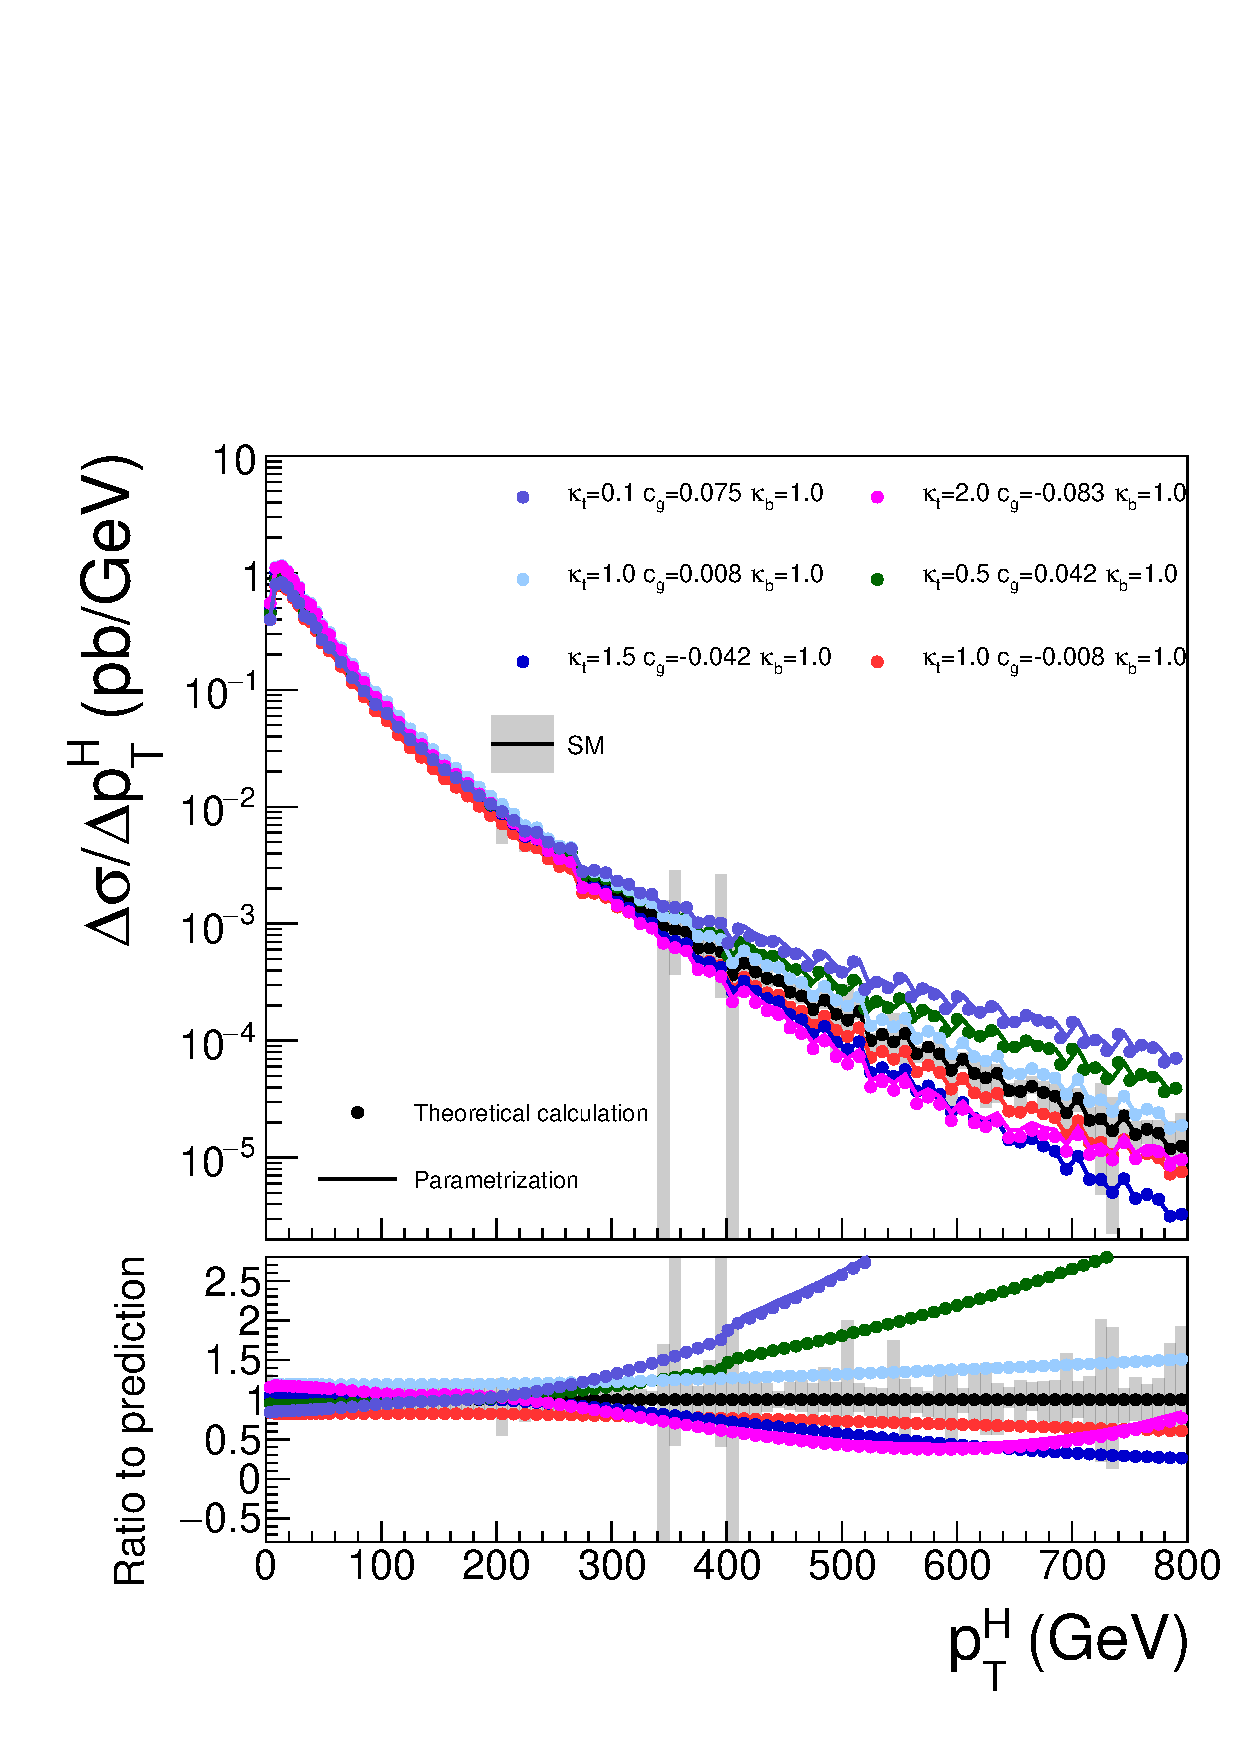
\includegraphics[width=\halflinewidth]{img/interpretation/other/varparcomp_ktcg.pdf}
    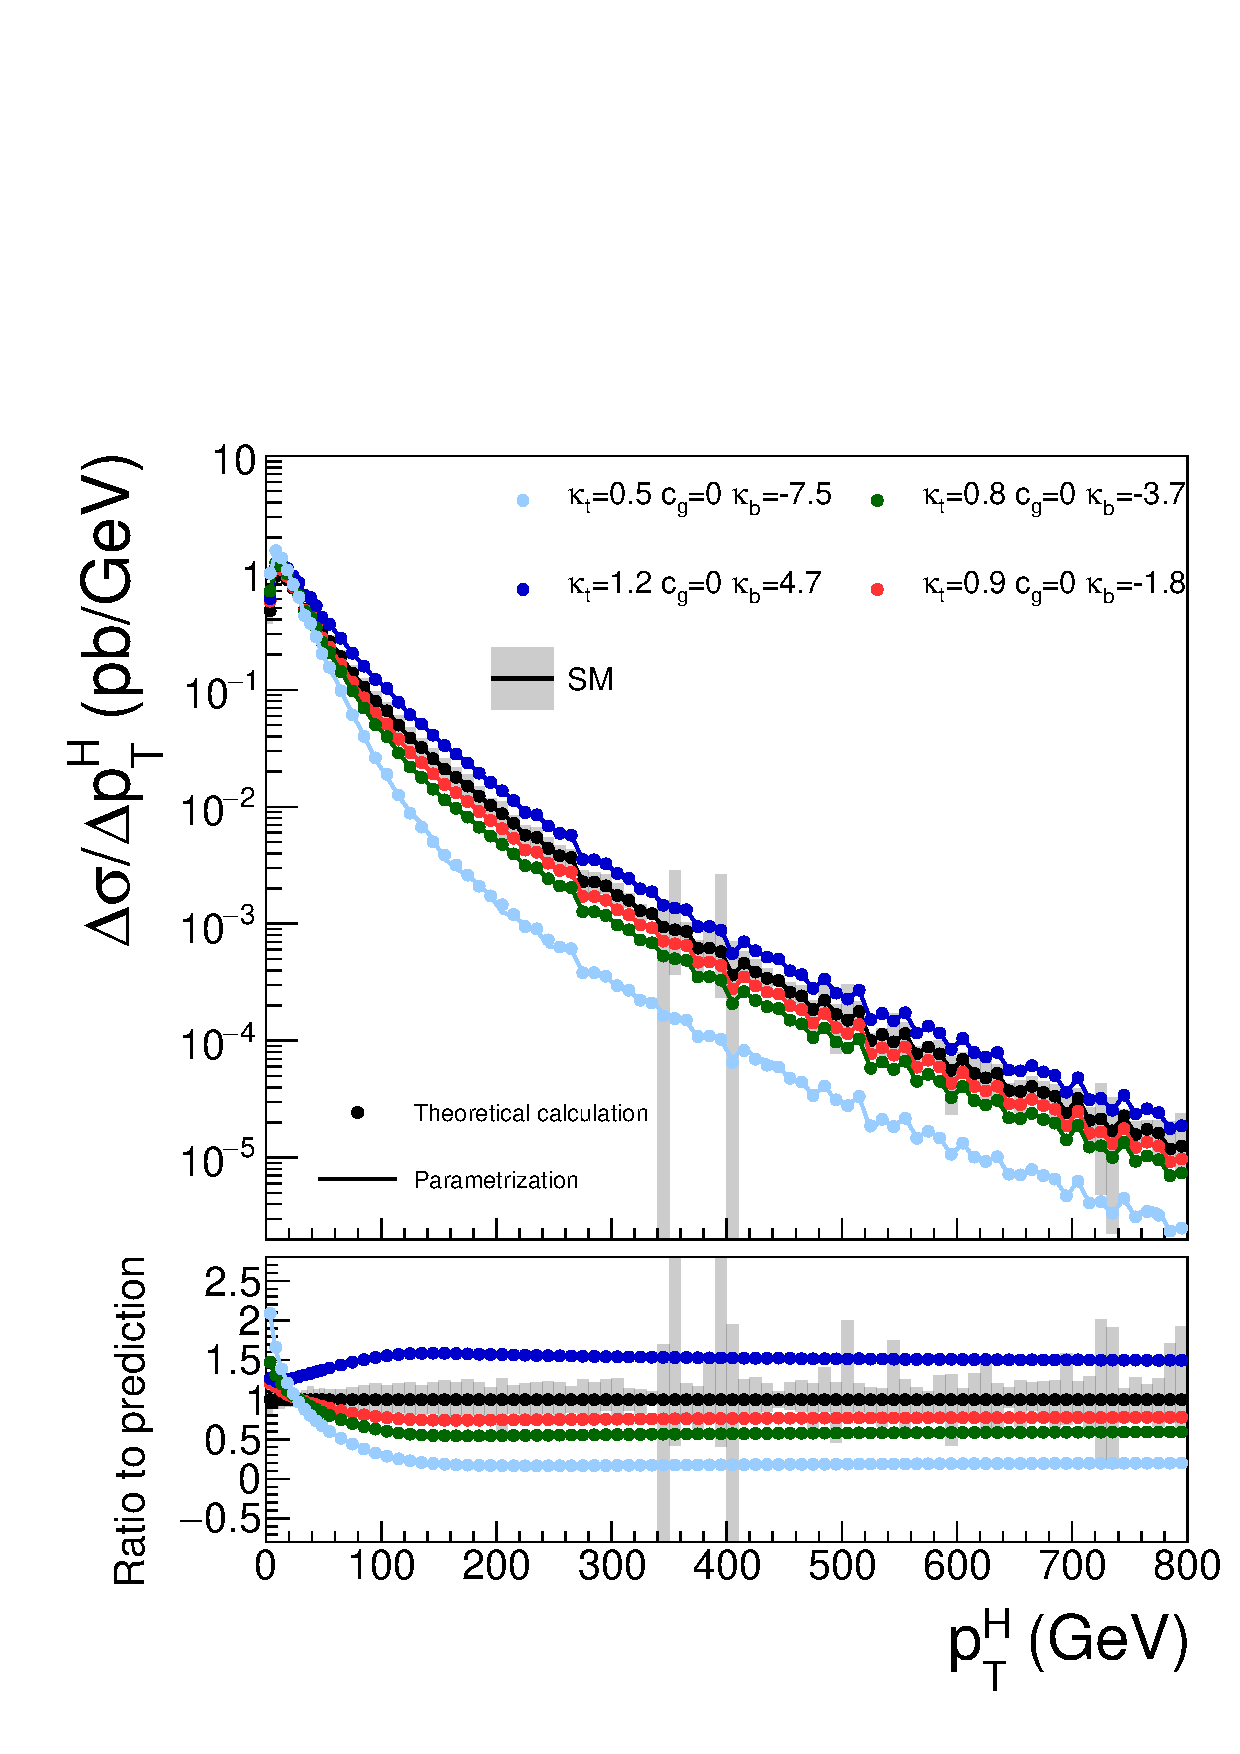
\includegraphics[width=\halflinewidth]{img/interpretation/other/varparcomp_ktkb.pdf}
    % 
    \caption{
        The predicted $\pth$ spectrum for simultaneous variations of $\kappat$ and $\cg$ (left) and $\kappat$ and $\kappab$ (right).
        % 
        The dots correspond to the theoretical calculations performed by the authors in Ref.~\cite{Grazzini:2017szg}, and the corresponding line shows the outcome of the parametrization of the theoretical calculations using a quadratic polynomial.
        % 
        The parametrization matches the exact calculations to a good approximation.
        % 
        The SM prediction is shown in black, with the gray bar indicating the uncertainty due to missing higher order corrections.
        }
    \label{fig:theories_ktcgkb}
  \end{center}
\end{figure}


For the spectra from Ref.~\cite{Bishara:2016jga} the statistical fluctuations are non-negligible, and the matrix inversion would translate the statistical noise to the coefficients in an amplified way.
% 
Instead, the coefficients are fitted to the set of precomputed spectra.
% 
The coefficients of the interference terms with the top quark are non-negligible, and are included in the fit; written out, Equation~(\ref{eq:kappa-parametrization}) for these spectra becomes
% 
\begin{linenomath*}
\begin{equation}
\begin{split}
\Delta\sigma
  & = A \kappab^2 + B \kappac^2 + C \kappab \kappac
    + D \kappat \kappab + E \kappat \kappac + F \kappat^2
  \\
  & = A \kappab^2 + B \kappac^2 + C \kappab \kappac
    + D \kappab + E \kappac + F
  \,,
\end{split}
\end{equation}
\end{linenomath*}
% 
where $\kappat$ is fixed to $1$.
% 
The parametrization and the precomputed spectra are shown for selected values of $\kappab$ and $\kappac$ in Fig.\ref{fig:theories_kbkc}.


\begin{figure}[hbtp]
  \begin{center}
    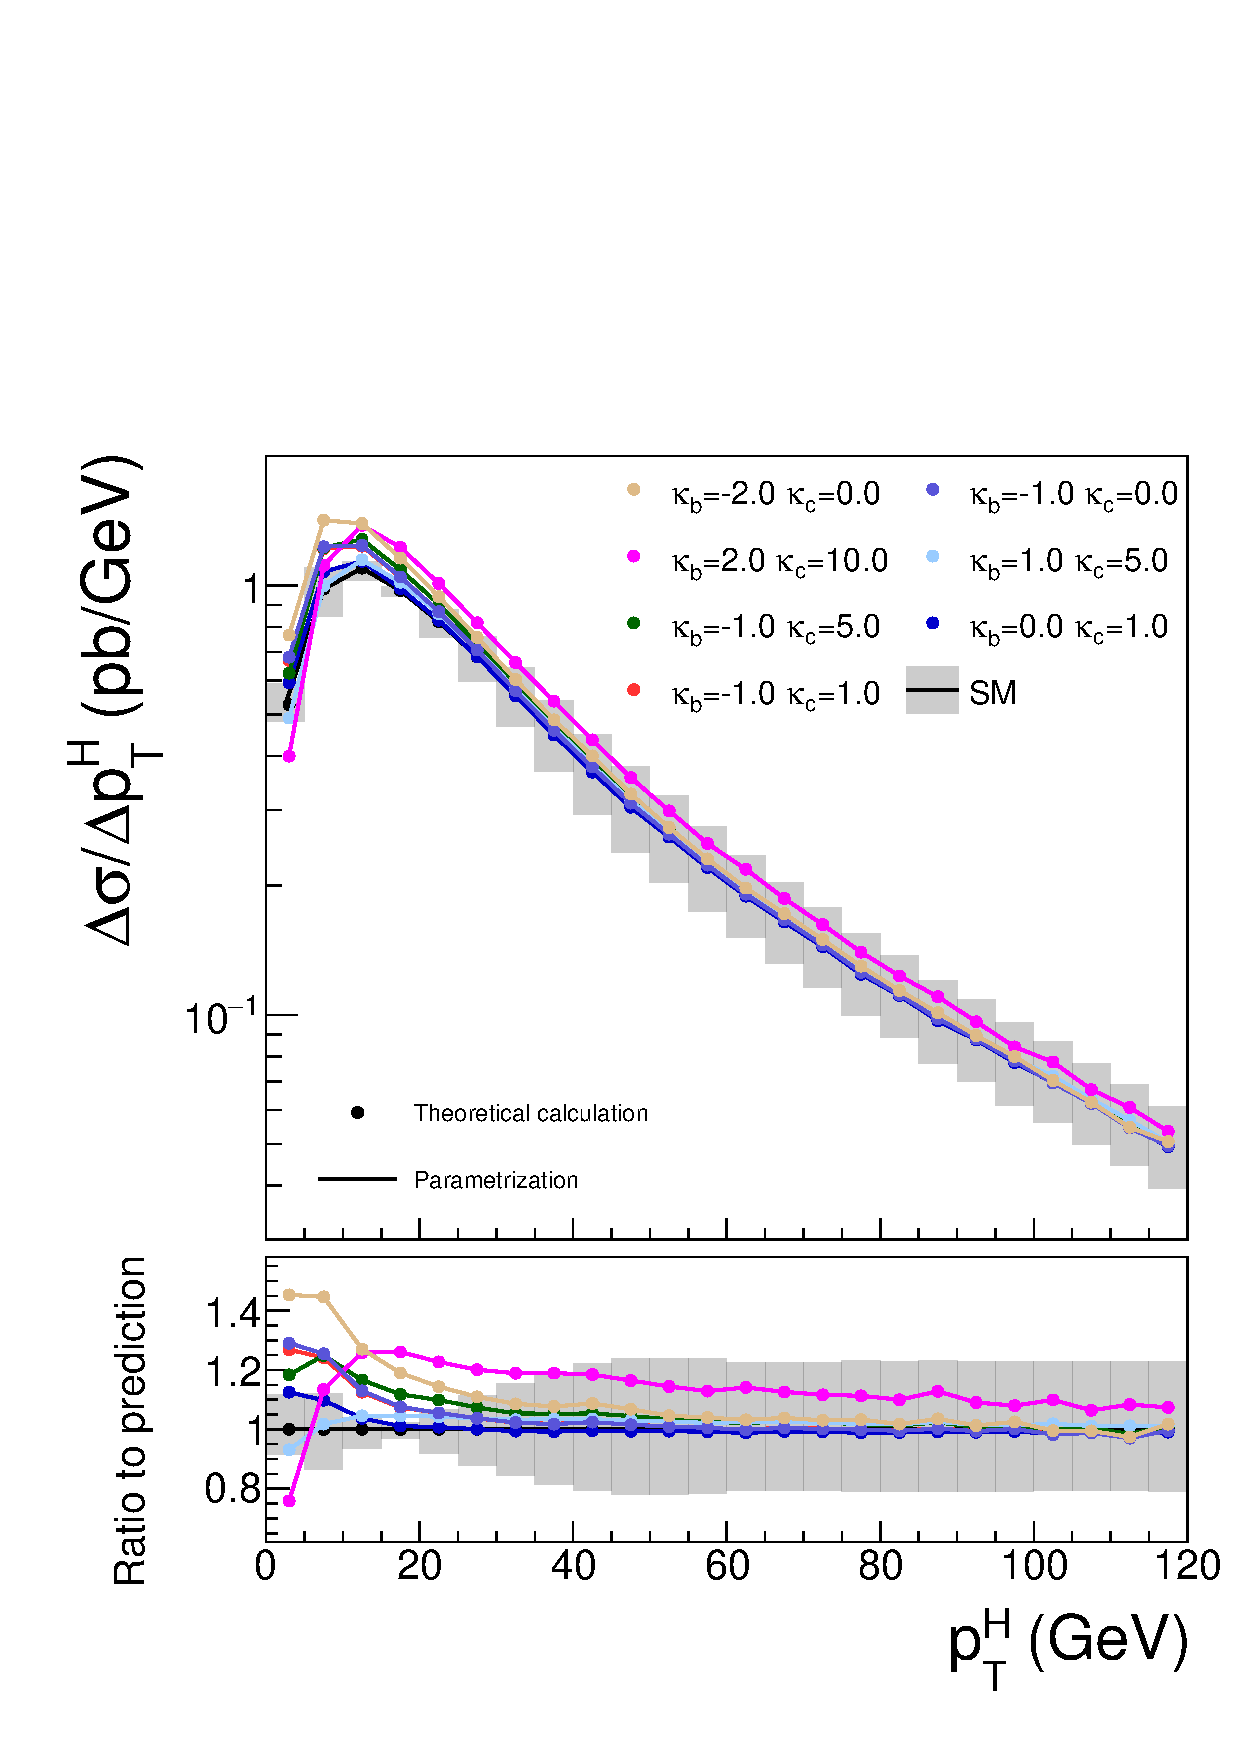
\includegraphics[width=\halflinewidth]{img/interpretation/other/varparcomp_kbkc.pdf}
    % 
    \caption{
        The predicted $\pth$ spectrum for simultaneous variations of $\kappab$ and $\kappac$.
        % 
        The dots correspond to the theoretical calculations performed by the authors in Ref.~\cite{Bishara:2016jga}, and the corresponding line shows the outcome of the parametrization of the theoretical calculations using a fitted quadratic polynomial.
        % 
        The parametrization matches the exact calculations to a good approximation.
        % 
        The SM prediction is shown in black, with the gray bar indicating the uncertainty due to missing higher order corrections.
        }
    \label{fig:theories_kbkc}
  \end{center}
\end{figure}


The shape can now be computed by inserting the parametrization of the differential cross section into Equation~(\ref{eq:interpretation-shape}).
% 
For variations of $\kappat$ and $\cg$, the shape becomes
% 
\begin{linenomath*}
\begin{equation}
\label{eq:interpretation-shape-ktcg}
\begin{split}
s^{\ggh}_i(\kappat, \cg)
        &=
        \frac
            {\Delta\sigma^{\ggh}_i(\kappat, \cg)}
            {\sum_j \Delta\sigma^{\ggh}_j(\kappat, \cg)}
            \\
        &=
        \frac
            {A_i \kappat^2 + B_i \cg^2 + C_i \kappat \cg}
            {
                \left(\sum_j A_j\right) \kappat^2
                + \left(\sum_j B_j\right) \cg^2
                + \left(\sum_j C_j\right) \kappat\cg
                }
            \\
        &= 
        \frac
            {A_i \frac{\kappat^2}{\cg^2} + B_i + C_i \frac{\kappat}{\cg}}
            {
                \left(\sum_j A_j\right) \frac{\kappat^2}{\cg^2}
                + \left(\sum_j B_j\right) 
                + \left(\sum_j C_j\right) \frac{\kappat}{\cg}
                }
            \\
        & = f(\frac{\kappat}{\cg})
\,,
\end{split}
\end{equation}
\end{linenomath*}
% 
where $A_i$, $B_i$, and $C_i$ are the coefficients of the parametrization in bin $i$.
% 
In other words, the shape of the $\pth$ spectrum via $\ggh$ is only a function of the ratio of $\kappat$ and $\cg$; it is invariant under any transformation
% 
\begin{linenomath*}
\begin{equation}
\label{eq:interpretation-ktcg-transform}
(\kappat, \cg) \to (c \cdot \kappat, c \cdot \cg)
\,,
\end{equation}
\end{linenomath*}
% 
where $c$ is a real-valued constant.
% 
The argument follows analogously for variations of $\kappat$ and $\kappab$.


For the variations of $\kappab$ and $\kappac$, the interference terms due to the top quark break the ratio-dependence observed in Equation~(\ref{eq:interpretation-shape-ktcg}).
% 
Only in the limit of large couplings these interference terms are negligible, and one obtains again a dependence on purely $\kappab/\kappac$:
% 
\begin{linenomath*}
\begin{equation}
\label{eq:interpretation-shape-kbkc}
\begin{split}
\lim_{\kappab,\,\kappac\to\infty} & s^{\ggh}_i(\kappab, \kappac) \\
        % 
        &=
        \lim_{\kappab,\,\kappac\to\infty}
        \frac
            {\Delta\sigma^{\ggh}_i(\kappab, \kappac)}
            {\sum_j \Delta\sigma^{\ggh}_j(\kappab, \kappac)}
            \\
        &=
        \lim_{\kappab,\,\kappac\to\infty}
        \frac
            {A_i \kappab^2 + B_i \kappac^2 + C_i \kappab \kappac
                + D_i \kappab + E_i \kappac + F_i
                }
            {
                \left(\sum_j A_j\right) \kappab^2
                + \left(\sum_j B_j\right) \kappac^2
                + \left(\sum_j C_j\right) \kappab\kappac
                + \left(\sum_j D_j\right) \kappab
                + \left(\sum_j E_j\right) \kappac
                + \left(\sum_j F_j\right)
                }
            \\
        &=
        \frac
            {A_i \frac{\kappab^2}{\kappac^2} + B_i + C_i \frac{\kappab}{\kappac}}
            {
                \left(\sum_j A_j\right) \frac{\kappab^2}{\kappac^2}
                + \left(\sum_j B_j\right) 
                + \left(\sum_j C_j\right) \frac{\kappab}{\kappac}
                }
            \\
        & = f(\frac{\kappab}{\kappac})
\,.
\end{split}
\end{equation}
\end{linenomath*}
% 
For the fits in this thesis however, the couplings never become large enough for the linear terms to be negligible.









